\subsection{Pneumatik}\label{sec:Pneumatik}
Um ein Vakuum zu erzeugen und um den Satelliten rütteln zu lassen, werden Pneumatik Teile benötig.
Pneumatik ist ein Bereich der Technik, der Druckluft nutzt, um mechanische Arbeit einfach zu verrichten. Es bietet eine vielseitige und sichere Methode für verschiedene Anwendungen wie Automatisierung, Maschinenbau und Fahrzeugtechnik. Durch die Verwendung von pneumatischen Aktuatoren wie Zylindern und Ventilen können Bewegungen gesteuert und automatisiert werden. Insgesamt ermöglicht Pneumatik eine effiziente und zuverlässige mechanische Leistung. Für die Teststation werden folgende Pneumatik Teile benötigt:
\vspace{3mm}
\begin{table}[H]
    \centering
    \begin{tabular}{ | c | c | } 
  \hline
   \textbf{Bezeichnung} & \textbf{Stückzahl}\\ 
  \hline
   Ventil 24 VDC & 1\\ 
  \hline
    Ventil 24 VDC, Druck justierbar & 1 \\ 
  \hline
  Vakuum Ejektor & 1 \\ 
  \hline
  Druckluft Kugel Vibrator & 1 \\ 
  \hline
\end{tabular}
    \caption{Stückliste Pneumatik}
\end{table}
\vspace{2mm}
Mit den beiden Ventil können wir die Luftzufuhr zu dem Vakuum Ejektor und dem Druckluft Kugel Vibrator steuern. Mit dem Vibrator können wir eine Rüttelplatte verwirklichen und können so den Satelliten auf Vibrationen testen. Die Pneumatik Teile wurden uns von der Firma Hefel Technik GmbH gesponsert, die spezialisiert auf Pneumatik und Automatisierungstechnik sind.\\
\newpage
\textbf{Komplette Zusammenschaltung Pneumatik}\\
\vspace{3mm}
\begin{figure}[H]
    \centering
    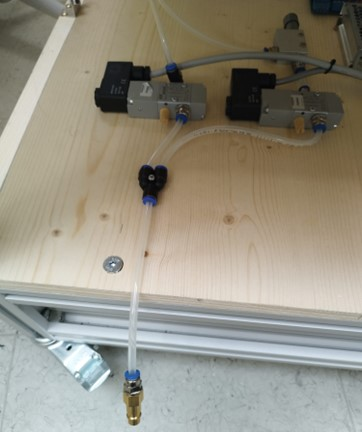
\includegraphics[scale=0.6]{image/zusammenpneumatik.jpg}
    \caption{Zusammenschaltung Pneumatik}
    \label{fig:enter-label}
\end{figure}
Das rechte Ventil ist für die Rüttelplatte und beim rechten ist direkt der Vakuum Ejektor angeschlossen. \\

\subsubsection{Ventil}
Das VY-83ELB00-T\autocite{Ventil} ist ein pneumatisches Ventil, das häufig in der Industrie eingesetzt wird, um den Durchfluss von Druckluft zu steuern. Mit diesem Ventil steuern wir die Rüttelplatte und den Vakuum Ejektor. So ein Ventil besteht aus einem elektromagnetischen Spulenmechanismus, der einen beweglichen Ventilspulenkern betätigt, um den Luftstrom zu öffnen oder zu schließen. Das VY-Solenoidventil bietet eine zuverlässige und präzise Steuerung des Luftstroms, was es ideal für Anwendungen in der Automatisierung, Maschinenbau und anderen industriellen Bereichen macht.\\
\vspace{3mm}
\begin{figure}[H]
    \centering
    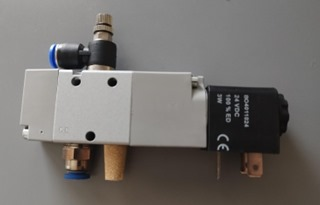
\includegraphics{image/ventil.jpeg}
    \caption{Ventil}
    \label{fig:enter-label}
\end{figure}
\vspace{3mm}
Steuern kann man das Ventil, in dem man eine Spannung anschließt. Werden 24V eingespeist, öffnet das Ventil und die Luft kann durchströmen. Sobald die Spannung entzogen wird, schließt sich das Ventil wieder. Die Spannungszufuhr wird mit einem Relais gesteuert.
\begin{figure}[H]
    \centering
    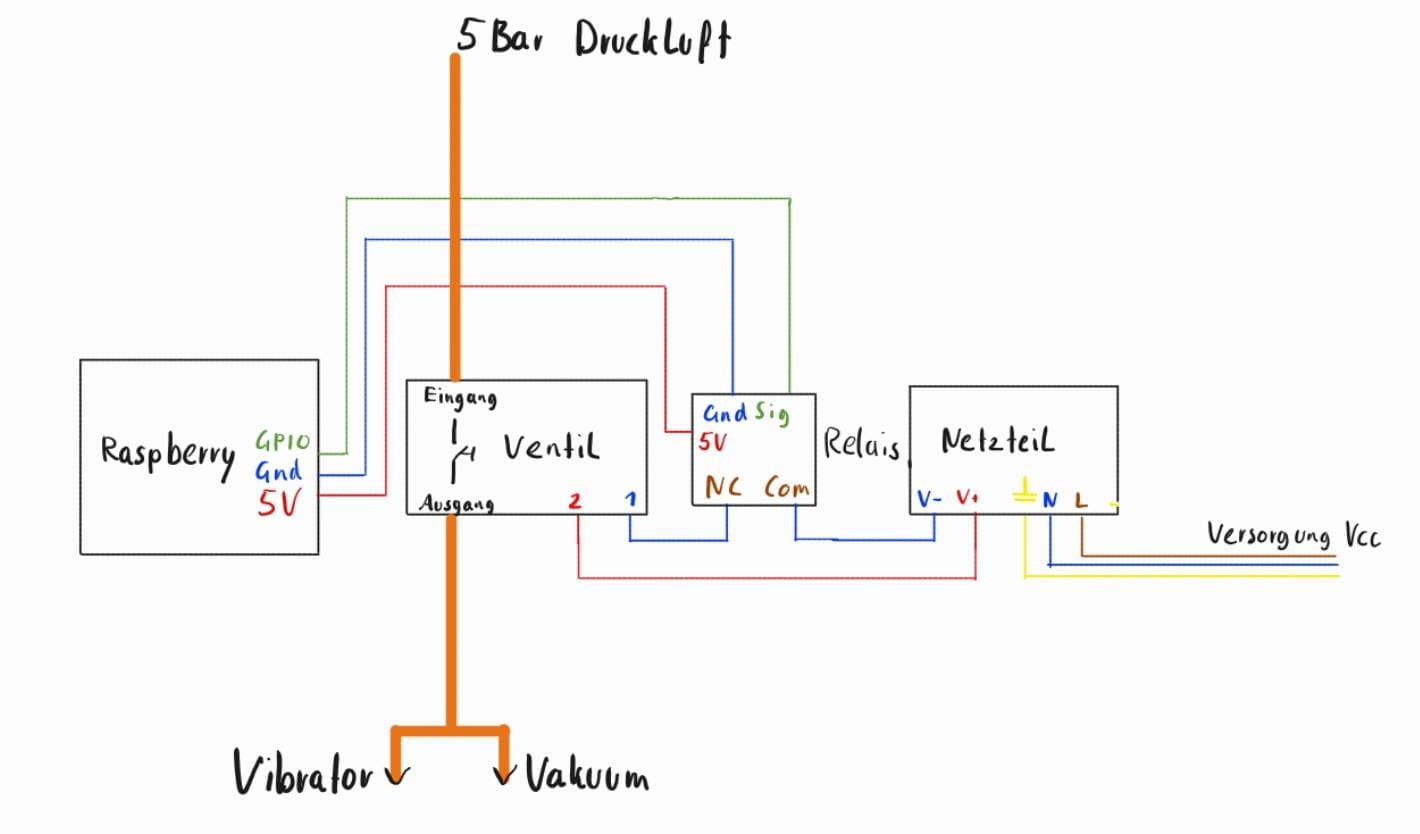
\includegraphics[scale=1.1]{image/zusammenschaltngventil.jpeg}
    \caption{Zusammenschaltung Ventil}
    \label{fig:enter-label}
\end{figure}

\subsubsection{Vakuum Ejektor}
Da wir den Satelliten in einem Vakuum testen müssen, benötigen wir ein Vakuum Erzeuger. Ein Vakuum ist ein physikalischer Zustand, der durch das Fehlen von Materie in einem bestimmten Bereich gekennzeichnet ist. Es ist ein Raum, der frei von Gasen, Flüssigkeiten oder Feststoffen ist. In einem Vakuum gibt es keinen atmosphärischen Druck, da kein Medium vorhanden ist, das diesen Druck ausüben könnte. Da der Weltraum nahezu leer von Materien ist und deshalb ein Vakuum ist, wird der Satellit auch auf diese Einflüsse getestet.\\
\vspace{3mm}
Ein Vakuum-Ejektor\autocite{VakuumEjektor} erzeugt ein Vakuum durch Absaugen von Luft oder Gas aus einem geschlossenen Raum. Dies geschieht durch Hochdruckluft, die durch eine Düse strömt und einen Unterdruck erzeugt. Vakuum-Ejektoren sind effizient, zuverlässig und erfordern wenig Wartung. Mit dem Ventil kann der Vakuum Ejektor gesteuert werden.\\
\vspace{3mm}
Wir haben uns für den Typ CV\autocite{VakuumEjektor} entschieden, da dieser haltbar und langlebig und langlebig ist, dieser Typ ist der beliebteste Ejektor.
Mit diesem kann ein Vakuumwert von - 0,58 oder  - 0,92 Bar erreicht werden.
\vspace{3mm}
\begin{figure}[H]
    \centering
    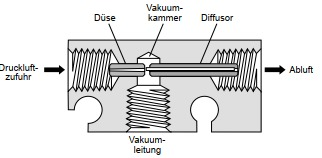
\includegraphics[scale=1.2]{image/vakuumejektor.jpeg}
    \caption{Skizze Vakuum-Ejektoren\autocite{VakuumEjektor}}
    \label{fig:enter-label}
\end{figure}
\vspace{3mm}
Der Satellit wird dann in eine Vakuum Glocke gegeben. Eine Vakuumglocke ist eine abgedichtete Glaskuppel, die in unserem Fall über den Satelliten platziert wird, um ein Vakuum zu erzeugen. Sie schützt den Satelliten vor äußeren Einflüssen wie Luft, Staub oder Feuchtigkeit und wird oft in Labors und Werkstätten verwendet, um eine kontrollierte Atmosphäre zu schaffen.
\begin{figure}[H]
    \centering
    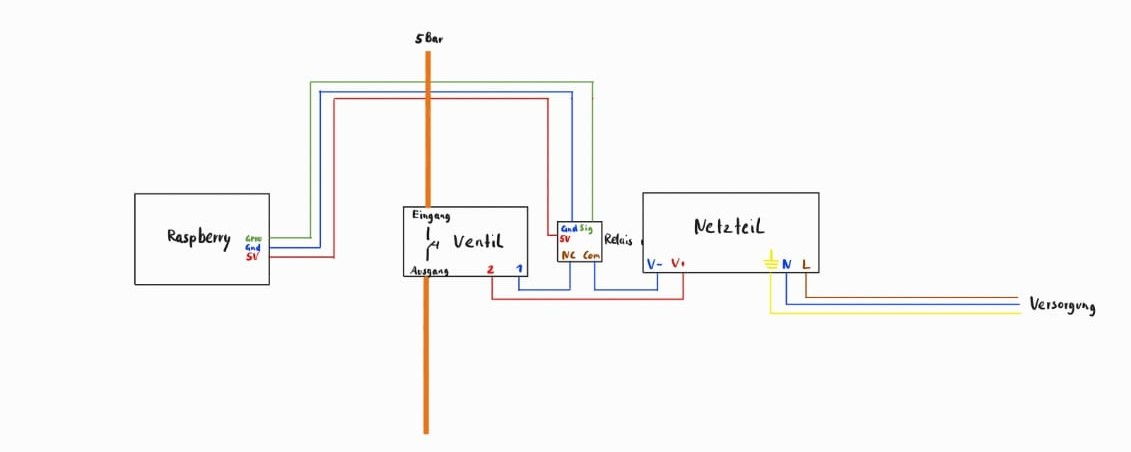
\includegraphics[scale=0.5]{image/vakummejektorzusammen.jpeg}
    \caption{Ejektor Zusammenschaltung}
    \label{fig:enter-label}
\end{figure}

\subsubsection{Druckluft Kugel Vibrator}
Ein pneumatischer Kugelvibrator ist ein Gerät, die verwendet wird, um Vibrationen zu erzeugen, indem Druckluft durch einen Hohlraum geleitet wird, der eine Kugel enthält. Hier ist eine Beschreibung, wie ein pneumatischer Kugelvibrator funktioniert:
Ein pneumatischer Kugelvibrator besteht aus einem Gehäuse, das eine oder mehrere Kugeln enthält, die sich frei bewegen können. Das Gehäuse hat Ein- und Auslassöffnungen, durch die Druckluft ein- und austreten kann. Die Zufuhr wird mit einem Ventil gesteuert.\\
Druckluft wird durch die Einlassöffnung in das Gehäuse geleitet, der Druck wird mit dem Ventil gesteuert. Diese Luftströmung erzeugt eine Druckdifferenz im Inneren des Gehäuses, die die Kugel oder Masse dazu bringt, sich zu bewegen.\\
\vspace{3mm}
Wenn die Druckluft in das Gehäuse strömt, dreht sich die Kugel im Inneren. Diese Bewegung erzeugt Vibrationen, die auf das umgebende Material oder die Maschine übertragen werden.\\
\vspace{3mm}
Die Intensität der Vibration kann durch die Steuerung des Luftdrucks und der Luftströmung gesteuert werden. Durch Anpassen dieser Parameter kann die Vibrationsstärke des Kugelvibrators angepasst werden.\\
\vspace{3mm}
\begin{figure}[H]
    \centering
    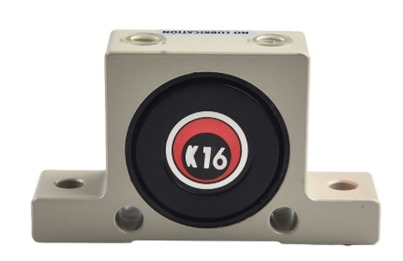
\includegraphics{image/vibration.jpeg}
    \caption{Druckluft Kugel Vibrator\autocite{PneumatischerVibrator}}
    \label{fig:enter-label}
\end{figure}
\subsubsection{Rüttelplatte}
Um den Druckluft Kugel Vibrator zu verwenden, muss eine Plattform gebaut werden, die beweglich ist, aber trotzdem fix verschraub bar ist.  Dazu sind sogenannt Schwingungsdämpfer nötig. Diese bestehen aus  Gummi und können mit M8 Schrauben befestigt werden. Auf die Plattform wird der Satellit platziert und kann durchgeschüttelt werden.
Die Rüttelplatte wird an den Dämpfungselementen mit einem Rest-Aluprofile verschraubt. \\
\vspace{3mm}
\begin{figure}[H]
    \centering
    \begin{subfigure}[b]{0.4\textwidth}
        \centering
        \includegraphics[width=\textwidth]{image/rüttelplatte1.jpeg}
        
        \label{fig:bild1}
    \end{subfigure}
    \hfill
    \begin{subfigure}[b]{0.47\textwidth}
        \centering
        \includegraphics[width=\textwidth]{image/rüttelplatte2.jpeg}
        
        \label{fig:bild2}
    \end{subfigure}
    \caption{Rüttelplatte}
    \label{fig:zwei_bilder}
\end{figure}
\vspace{3mm}
Da die Schrauben von den Schwingungsdämpfern zu kurz sind, werden sie an einer Aluplatte befestigt. Diese Platte ist mit dem Vibrator verschraubt. Eine zweite Aluplatte ist notwendig, um den Satelliten drauf zu stellen. Die Schrauben werden mit Schraubkleber beschmiert, da sie sich sonst bei ständigen Vibrationen lösen.